\chapter{Signaturas de caminos: el orden de los movimientos}\label{cap:signaturas}

Los indicadores clásicos resumen una serie con niveles (medias, máximos, volatilidad). La
\textbf{signatura} de un camino, que viene de la teoría de \emph{rough paths} de T.~Lyons, resume
también el \emph{orden} en que se mueven varias series a la vez. En investigación cuantitativa se usa
como fuente de rasgos para modelos lineales, para medir qué activo se mueve antes y para problemas de
ejecución. Este capítulo es una ampliación opcional: explica qué es, qué propiedades tiene de verdad
(en particular, qué significa que sea «invariante» y qué no) y la implementa en
\py{trader.signature}. Las demostraciones están en la guía teórica del repositorio (capítulo de rough
paths) y en las referencias de la bibliografía.

\section{Motivación: dos caminos con las mismas rentabilidades}
Supón dos activos A y B que suben un 1~\% cada uno en una sesión. En el camino~1 sube primero A y
después B; en el camino~2, al revés. El incremento total es idéntico, la volatilidad también, y una
estrategia que mire sólo rentabilidades de cierre a cierre no distingue los dos casos. Sin embargo, si A
se mueve sistemáticamente antes que B, eso es información operable (y un riesgo si estás cubriendo B
con A). La signatura es una forma sistemática de capturar ese orden.

\section{Definición y cálculo}
Sea $X:[0,T]\to\mathbb R^d$ un camino (por ejemplo, $d$ log-precios). Su signatura es la sucesión de
integrales iteradas
\begin{equation}\label{eq:signatura}
S^{i}=\int_0^T dX^i_s,\qquad
S^{ij}=\iint_{0<s<u<T} dX^i_s\,dX^j_u,\qquad
S^{ijk}=\iiint_{0<s<u<v<T} dX^i_s\,dX^j_u\,dX^k_v,\ \dots
\end{equation}
El nivel~1 son los incrementos; el nivel~2 contiene, además de productos de incrementos, el
\emph{área de Lévy} $A^{ij}=\tfrac12(S^{ij}-S^{ji})$; el nivel~3 añade información sobre el orden de
tres movimientos. Truncada en el nivel $m$, tiene $d+d^2+\dots+d^m$ términos.

\paragraph{Cálculo exacto con datos discretos.} Se unen los datos con segmentos rectos. Para un único
segmento de incremento $\Delta$, la signatura es la exponencial tensorial:
$(\Delta,\ \tfrac12\Delta^{\otimes2},\ \tfrac16\Delta^{\otimes3})$. Para concatenar dos tramos se usa la
\textbf{identidad de Chen}: $S(X\ast Y)=S(X)\otimes S(Y)$, es decir,
\begin{equation}\label{eq:chen}
S^{(2)}(X\ast Y)=S^{(2)}(X)+S^{(1)}(X)\otimes S^{(1)}(Y)+S^{(2)}(Y),
\end{equation}
y análogamente en el nivel~3. Con incrementos $\Delta_k$ y sumas previas $C_k=\sum_{j<k}\Delta_j$ queda
$S^{(2)}=\sum_k\big(C_k\otimes\Delta_k+\tfrac12\Delta_k^{\otimes2}\big)$, que \py{signature.signature}
calcula vectorizado sobre lotes de caminos o ventanas.

\paragraph{Identidad de barajado.} Los productos de términos de la signatura son combinaciones lineales
de términos de nivel superior; en el nivel~2, $S^iS^j=S^{ij}+S^{ji}$. Por eso la parte simétrica de
$S^{(2)}$ no aporta nada nuevo: $S^{(2)}=\tfrac12 S^{(1)}\otimes S^{(1)}+A$, y la
\emph{log-signatura} de nivel~2 es simplemente $(S^{(1)},A)$ (\py{signature.log\_signature2}). Esta
propiedad hace que una función \emph{lineal} de la signatura sea muy expresiva: con el tiempo como
canal adicional, cualquier función continua del camino se aproxima tan bien como se quiera por funciones
lineales de la signatura truncada (\emph{universalidad}).

\section{Invarianzas: qué ve y qué no ve la signatura}
\paragraph{Reparametrización.} Si $\varphi$ es un cambio de reloj creciente, el camino $X\circ\varphi$
recorre los mismos puntos a otra velocidad, y
\begin{equation}
S(X\circ\varphi)=S(X).
\end{equation}
Para datos de mercado esto significa que pausas, ticks repetidos, muestreo irregular o un ritmo de
llegada variable \emph{del mismo camino} no cambian los rasgos. Es la propiedad a la que se refiere la
expresión «invarianza frente a la latencia»: si una fuente de datos entrega los mismos precios en el
mismo orden pero con retrasos variables, la signatura de cada serie es la misma. Además, la signatura
es invariante por traslación (no depende del nivel de partida) y, salvo tramos que se deshacen sobre sí
mismos, determina el camino (Hambly y Lyons, 2010).

\begin{table}[h]\centering\small
\begin{tabularx}{\textwidth}{Xll}
\toprule
Cambio en los datos & ¿Cambia la signatura? & Comentario \\ \midrule
Pausas, ticks repetidos, ritmo de llegada & No & reparametrización \\
Subdividir un tramo recto & No & reparametrización \\
Sumar una constante a los precios & No & traslación \\
Retraso de un activo respecto a otro & \textbf{Sí} & lo mide el área de Lévy (\S\ref{sec:levy}) \\
Movimiento rápido frente a lento, con canal de tiempo & \textbf{Sí} & \py{signature.add\_time} \\
Perder puntos intermedios (muestreo más grueso) & \textbf{Sí}, en general & otro camino lineal a trozos \\
Latencia de tus órdenes & No aplica & es un coste de ejecución \\
\bottomrule
\end{tabularx}
\caption{Lo que la signatura ignora y lo que no (comprobado en \py{tests/test\_signature.py}).}
\end{table}

\begin{aviso}[La signatura no hace inmune a la latencia]
La invarianza es una propiedad de los \emph{rasgos}, no de la estrategia. Si tus órdenes llegan tarde
pagas el deslizamiento igual (capítulo~\ref{cap:micro}). Y un retraso \emph{relativo} entre dos activos
no se ignora: aparece en el área de Lévy, lo que es útil para detectarlo pero también puede crear
señales falsas si los dos activos cierran a horas distintas. Por último, ignorar el ritmo tiene un
coste: la velocidad del mercado (volatilidad por unidad de tiempo) importa, y para recuperarla hay que
añadir el tiempo como canal, con lo que se pierde la invarianza.
\end{aviso}

\section{Transformación lead-lag y variación cuadrática}
La signatura de un solo canal no ve la volatilidad: $S^{11}=\tfrac12(S^1)^2$ depende sólo del
incremento. La \textbf{transformación lead-lag} (\py{signature.lead\_lag}) duplica la serie en una
copia adelantada y otra retrasada: primero se mueve la adelantada y luego la retrasada la alcanza
(figura~\ref{fig:signaturas}, izquierda). El área de Lévy entre ambas copias es exactamente la mitad
de la variación cuadrática:
\begin{equation}\label{eq:leadlag}
A^{\text{lead},\text{lag}}=\tfrac12\sum_k(\Delta x_k)^2 .
\end{equation}
Así la varianza realizada aparece en el nivel~2 sin calcularla a mano, y los niveles superiores capturan
momentos de orden mayor y su relación con la dirección del precio.

\section{Área de Lévy: quién se mueve primero}\label{sec:levy}
Para dos canales, $A^{12}=\tfrac12\int(X^1\,dX^2-X^2\,dX^1)$ es el área con signo entre el camino y la
cuerda que une sus extremos: si se recorre un cuadrado unidad en sentido antihorario, $A^{12}=1$. Si
$X^1$ sube y \emph{después} sube $X^2$, el área es positiva; si es al revés, negativa. Por eso
$A^{12}>0$ indica que el canal~1 tiende a moverse antes.

Calculada sobre todo el histórico, el área es muy ruidosa (su desviación típica crece como la propia
señal). \py{signature.lead\_lag\_score} estandariza las rentabilidades, las acumula en ventanas sin
solape de $w$ sesiones y promedia el área normalizada por $(w-1)/2$. Su esperanza es
\begin{equation}\label{eq:score}
\E[\text{puntuación}]=\sum_{h=1}^{w-1}\frac{w-h}{w-1}\big[\rho_{x\to y}(h)-\rho_{y\to x}(h)\big],
\qquad \rho_{x\to y}(h)=\operatorname{corr}(r^x_t,r^y_{t+h}),
\end{equation}
que se reduce a $\rho_{x\to y}(1)-\rho_{y\to x}(1)$ si sólo hay desfase de un periodo. El error típico
sale de la dispersión entre ventanas. La figura~\ref{fig:signaturas} (derecha) lo comprueba con
$r^B_t=\rho\,r^A_{t-1}+\sqrt{1-\rho^2}\,\varepsilon_t$: la puntuación estimada sigue la recta $\rho$.
\begin{lstlisting}
python scripts/calculadoras.py liderazgo --csv datos/cierres.csv --a SPY --b EWJ
\end{lstlisting}

\begin{figure}[h]\centering
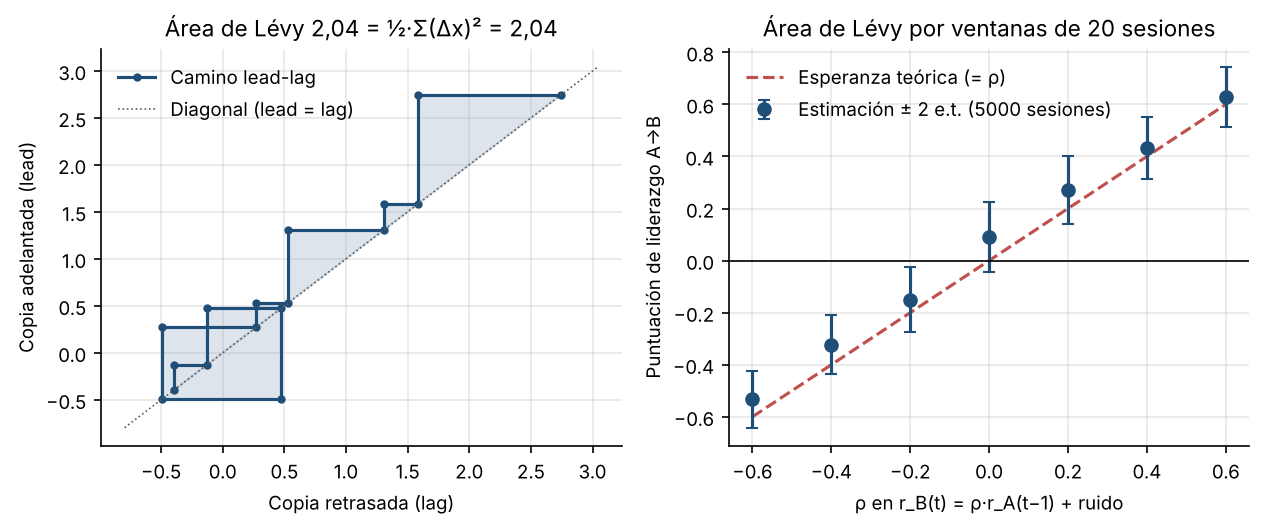
\includegraphics[width=\textwidth]{f12_signaturas}
\caption{Izquierda: camino lead-lag de 9 precios; el área sombreada es la mitad de la variación
cuadrática~\eqref{eq:leadlag}. Derecha: puntuación de liderazgo~\eqref{eq:score} frente al valor teórico.}
\label{fig:signaturas}
\end{figure}

\begin{practica}[Cierres asíncronos]
Con cierres diarios, un mercado que cierra antes (Tokio) parece «seguir» a uno que cierra después
(Nueva York) el día anterior: es un artefacto del horario, no una ventaja. Lo mismo ocurre con activos
poco líquidos cuyo último precio es antiguo (\emph{precios rancios}), que además hacen que la correlación
medida baje al aumentar la frecuencia (efecto Epps). Antes de operar un liderazgo, compruébalo con
precios tomados a la misma hora y descuenta costes: los desfases que se ven en datos diarios suelen
estar ya arbitrados en datos intradía. Para covarianzas con datos asíncronos, el estimador de
Hayashi--Yoshida es la referencia.
\end{practica}

\section{Una estrategia lineal sobre la signatura}
\py{signature.window\_features} construye, para cada sesión y con datos sólo hasta ella, el camino de
la ventana de $w$ sesiones: tiempo, log-precio relativo dividido por la volatilidad de la ventana y su
transformación lead-lag. Se calcula la signatura (nivel~2: 10 rasgos; nivel~3: 36, una vez quitados los
términos de tiempo puro, que son constantes). \py{signature.sig\_momentum} (y
\py{backtest.signature\_momentum}) ajusta una regresión \emph{ridge} de la rentabilidad del día
siguiente sobre esos rasgos, con reestimación walk-forward (capítulo~\ref{cap:backtest}): cada $63$
sesiones se reajusta con las $500$ anteriores cuyo resultado ya se conoce, y la posición es el signo de
la predicción.
\begin{lstlisting}
python scripts/backtest.py --estrategia sig --ventana 20 --coste 2
\end{lstlisting}
Los tests comprueban que no hay look-ahead, que con rentabilidades autocorrelacionadas (AR(1) con
$\phi=0{,}3$) la estrategia gana fuera de muestra y, por el script, que sobre un paseo aleatorio no
encuentra ventaja: con los datos sintéticos por defecto su Sharpe es negativo, como debe ser.

\paragraph{Extensiones en la literatura.} Futter, Horvath y Wiese (2023) formulan la cartera de
media-varianza con señales exógenas como un funcional lineal de la signatura y obtienen la solución
explícita en función de la signatura esperada. Kalsi, Lyons y Pérez Arribas (2020) resuelven la
ejecución óptima buscando la velocidad de negociación entre funciones lineales de la signatura.

\section{Límites}
\begin{itemize}
\item \textbf{Dimensión.} Con $d$ canales y nivel $m$ hay $\sim d^m$ rasgos: con 5 activos y nivel~3,
  155. Sin regularización (ridge, lasso) y validación fuera de muestra, el sobreajuste está
  garantizado (capítulo~\ref{cap:backtest}).
\item \textbf{Interpolación.} Con datos discretos la signatura depende de cómo se unan los puntos
  (lineal, lead-lag, escalonado). Elige un esquema y mantenlo.
\item \textbf{No estacionariedad.} Los rasgos son estables; la relación entre rasgos y rentabilidad
  futura, no. Reestimar y medir la degradación es obligatorio.
\item \textbf{Normalización.} Sin dividir por la escala de la ventana, los términos de nivel $m$ escalan
  como la volatilidad elevada a $m$ y dominan los regímenes volátiles.
\item \textbf{Evidencia.} La teoría es sólida; la evidencia publicada de rentabilidad fuera de muestra
  con datos reales y costes es todavía escasa. Trátalo como una herramienta de investigación.
\end{itemize}

\begin{clave}
La signatura es una forma compacta y con buena teoría de describir el \emph{orden} de los movimientos
de varias series. Ignora el ritmo al que llegan los datos de cada serie, pero sí registra el desfase
entre series; eso la hace útil para medir liderazgo y como entrada de modelos lineales regularizados.
No es una ventaja en sí misma.
\end{clave}

\begin{ejercicios}
\begin{enumerate}
\item Comprueba con \py{signature.signature} que la signatura de un camino no cambia al repetir puntos,
  y que sí cambia con \py{signature.add\_time}.
\item Calcula con \py{signature.levy\_area} el área de un rectángulo de lados 2 y 3 recorrido en
  sentido horario. ¿Qué signo tiene?
\item Ejecuta \py{calculadoras.py liderazgo} con cierres de un ETF europeo y uno estadounidense. ¿El
  resultado se mantiene si usas precios de la misma hora?
\item Compara \py{backtest.py --estrategia sig} con \py{--estrategia sma} sobre tus datos, con costes de
  2~pb, y cuenta cuántas variantes (ventana, nivel) has probado antes de quedarte con una.
\end{enumerate}
\end{ejercicios}
